Practical part consists of applying and implementing EKF (Extended Kalman Filter) for estimation of 3D position in space, writing a simulation to validate the filter implementation, tuning KF (Kalman Filter) parameters (mainly evaluating covariances) by real-world experiments, testing out whole system and evaluating localization accuracy.

\subsection{Localization}

Due to sensor measurement noise state estimator is necessary. Thus Kalman filter will be implemented and deployed to track agents position assuming noisy observations of distance. Before going into details it's important to think about state evolution and observation models because Kalman filter assumes both to be linear. During project constant velocity model will be used, described by:
% TODO: equation

which is linear by itself. However, Euclidean distance measurement model (from beacon to agent) has non-linearity due to the \emph{norm}:
$$
    \Vert\boldsymbol{x}-\boldsymbol{b}\Vert_2 = \sqrt{{\left(\mathrm{b_x}-x\right)}^2+{\left(\mathrm{b_y}-y\right)}^2+{\left(\mathrm{b_z}-z\right)}^2}
$$
where $\boldsymbol{x} = (x,y,z)$ is vector representing agents position and $\boldsymbol{b} = (b_x,b_y,b_z)$ is position of one visible (in radio communication sense) beacon in space. This is where EKF comes into play, the method proposes to use linearized version of non-linear function by taking it's Jacobian and assuming that linearized model representation around a small deviation neighborhood holds true and usa that in place of the measurement matrix $\boldsymbol{H}$. This will be described later but, in short, one can take partial derivatives of the function with respect to each agent's position dimension and evaluate them at current state estimate. For instance:
$$
    \frac{\partial h(x)}{\partial x} = \frac{x-\mathrm{b_x}}{\sqrt{{\left(\mathrm{b_x}-x\right)}^2+{\left(\mathrm{b_y}-y\right)}^2+{\left(\mathrm{b_z}-z\right)}^2}}
$$

General discrete time EKF is defined as described in the following paragraphs. Starting with notation: $\hat{\mathbf{x}}_{k \mid k-1}$ represents the estimate of $\mathbf{x}$ at time instance $k$ given observations up to and including at time $k-1$. \smallskip

\textbf{Prediction step} \smallskip
$$\hat{\boldsymbol{x}}_{k \mid k-1}=f\left(\hat{\boldsymbol{x}}_{k-1 \mid k-1}, \boldsymbol{u}_k\right)$$
$$\boldsymbol{P}_{k \mid k-1}=\boldsymbol{F}_k \boldsymbol{P}_{k-1 \mid k-1} \boldsymbol{F}_k^T+\boldsymbol{Q}_k$$

\textbf{Update step} \smallskip
$$\tilde{\boldsymbol{y}}_k=\boldsymbol{z}_k-h\left(\hat{\boldsymbol{x}}_{k \mid k-1}\right)$$
$$\boldsymbol{S}_k=\boldsymbol{H}_k \boldsymbol{P}_{k \mid k-1} \boldsymbol{H}_k^T+\boldsymbol{R}_k$$
$$\boldsymbol{K}_k=\boldsymbol{P}_{k \mid k-1} \boldsymbol{H}_k^T \boldsymbol{S}_k^{-1}$$
$$\hat{\boldsymbol{x}}_{k \mid k}=\hat{\boldsymbol{x}}_{k \mid k-1}+\boldsymbol{K}_k \tilde{\boldsymbol{y}}_k$$
$$\boldsymbol{P}_{k \mid k}=\left(\boldsymbol{I}-\boldsymbol{K}_k \boldsymbol{H}_k\right) \boldsymbol{P}_{k \mid k-1}$$
where state transition and measurement matrices are partial derivatives (\emph{Jacobians}) of state evolution and observation model functions. In constant velocity case $\boldsymbol{f}(\boldsymbol{x})$ is already linear so that part can be discarded.
$$
    \begin{aligned}
        \boldsymbol{F}_k & =\left.\frac{\partial f}{\partial \boldsymbol{x}}\right|_{\hat{\boldsymbol{x}}_{k-1 \mid k-1}, \boldsymbol{u}_k} \\
        \boldsymbol{H}_k & =\left.\frac{\partial h}{\partial \boldsymbol{x}}\right|_{\hat{\boldsymbol{x}}_{k \mid k-1}}
    \end{aligned}
$$
% TODO: numerical example, at least Jacobian ?
% TODO: KF reference?

Distance measurement Jacobian can be computed in code by:
\begin{python}
def dist_jac(x_op, beacons):
    H = np.zeros((len(beacons), len(x_op)))
    for i, b in enumerate(beacons):
        H[i][:3] = ((x_op[:3] - b.get_pos()) \
            / np.linalg.norm(x_op[:3] - b.get_pos())).T
    return H
\end{python}
% doesn't stay formatted as i wish if i wrap it :'( despair
% \begin{figure}
%     \caption{Distance Jacobian $\boldsymbol{H} computation.$}
%     \label{code:distJ}
% \end{figure}
function takes in agent position at time $k-1$, beacon list and return partial derivatives of state variables with respect to each of the beacons. It's assumed that beacon number is fixed to 4.

\subsection{Simulation experiments}

Figure \ref{fig:sim} shows a trail run in simulation. The setup is running EKF described in previous section on noisy measurement. Noise is provided by adding a random sample from Gaussian distribution to each distance measurement at every timestamp. Big $X$ is marking the start of a trajectory, $GT$ line is ground truth trajectory generated by applying state transition matrix at each instant of time (moving at arbitrary speeds to cover a rectangle), blue path is the predicted one and lastly the numbered dots represent beacons arbitrarily placed in space.
\begin{figure}
    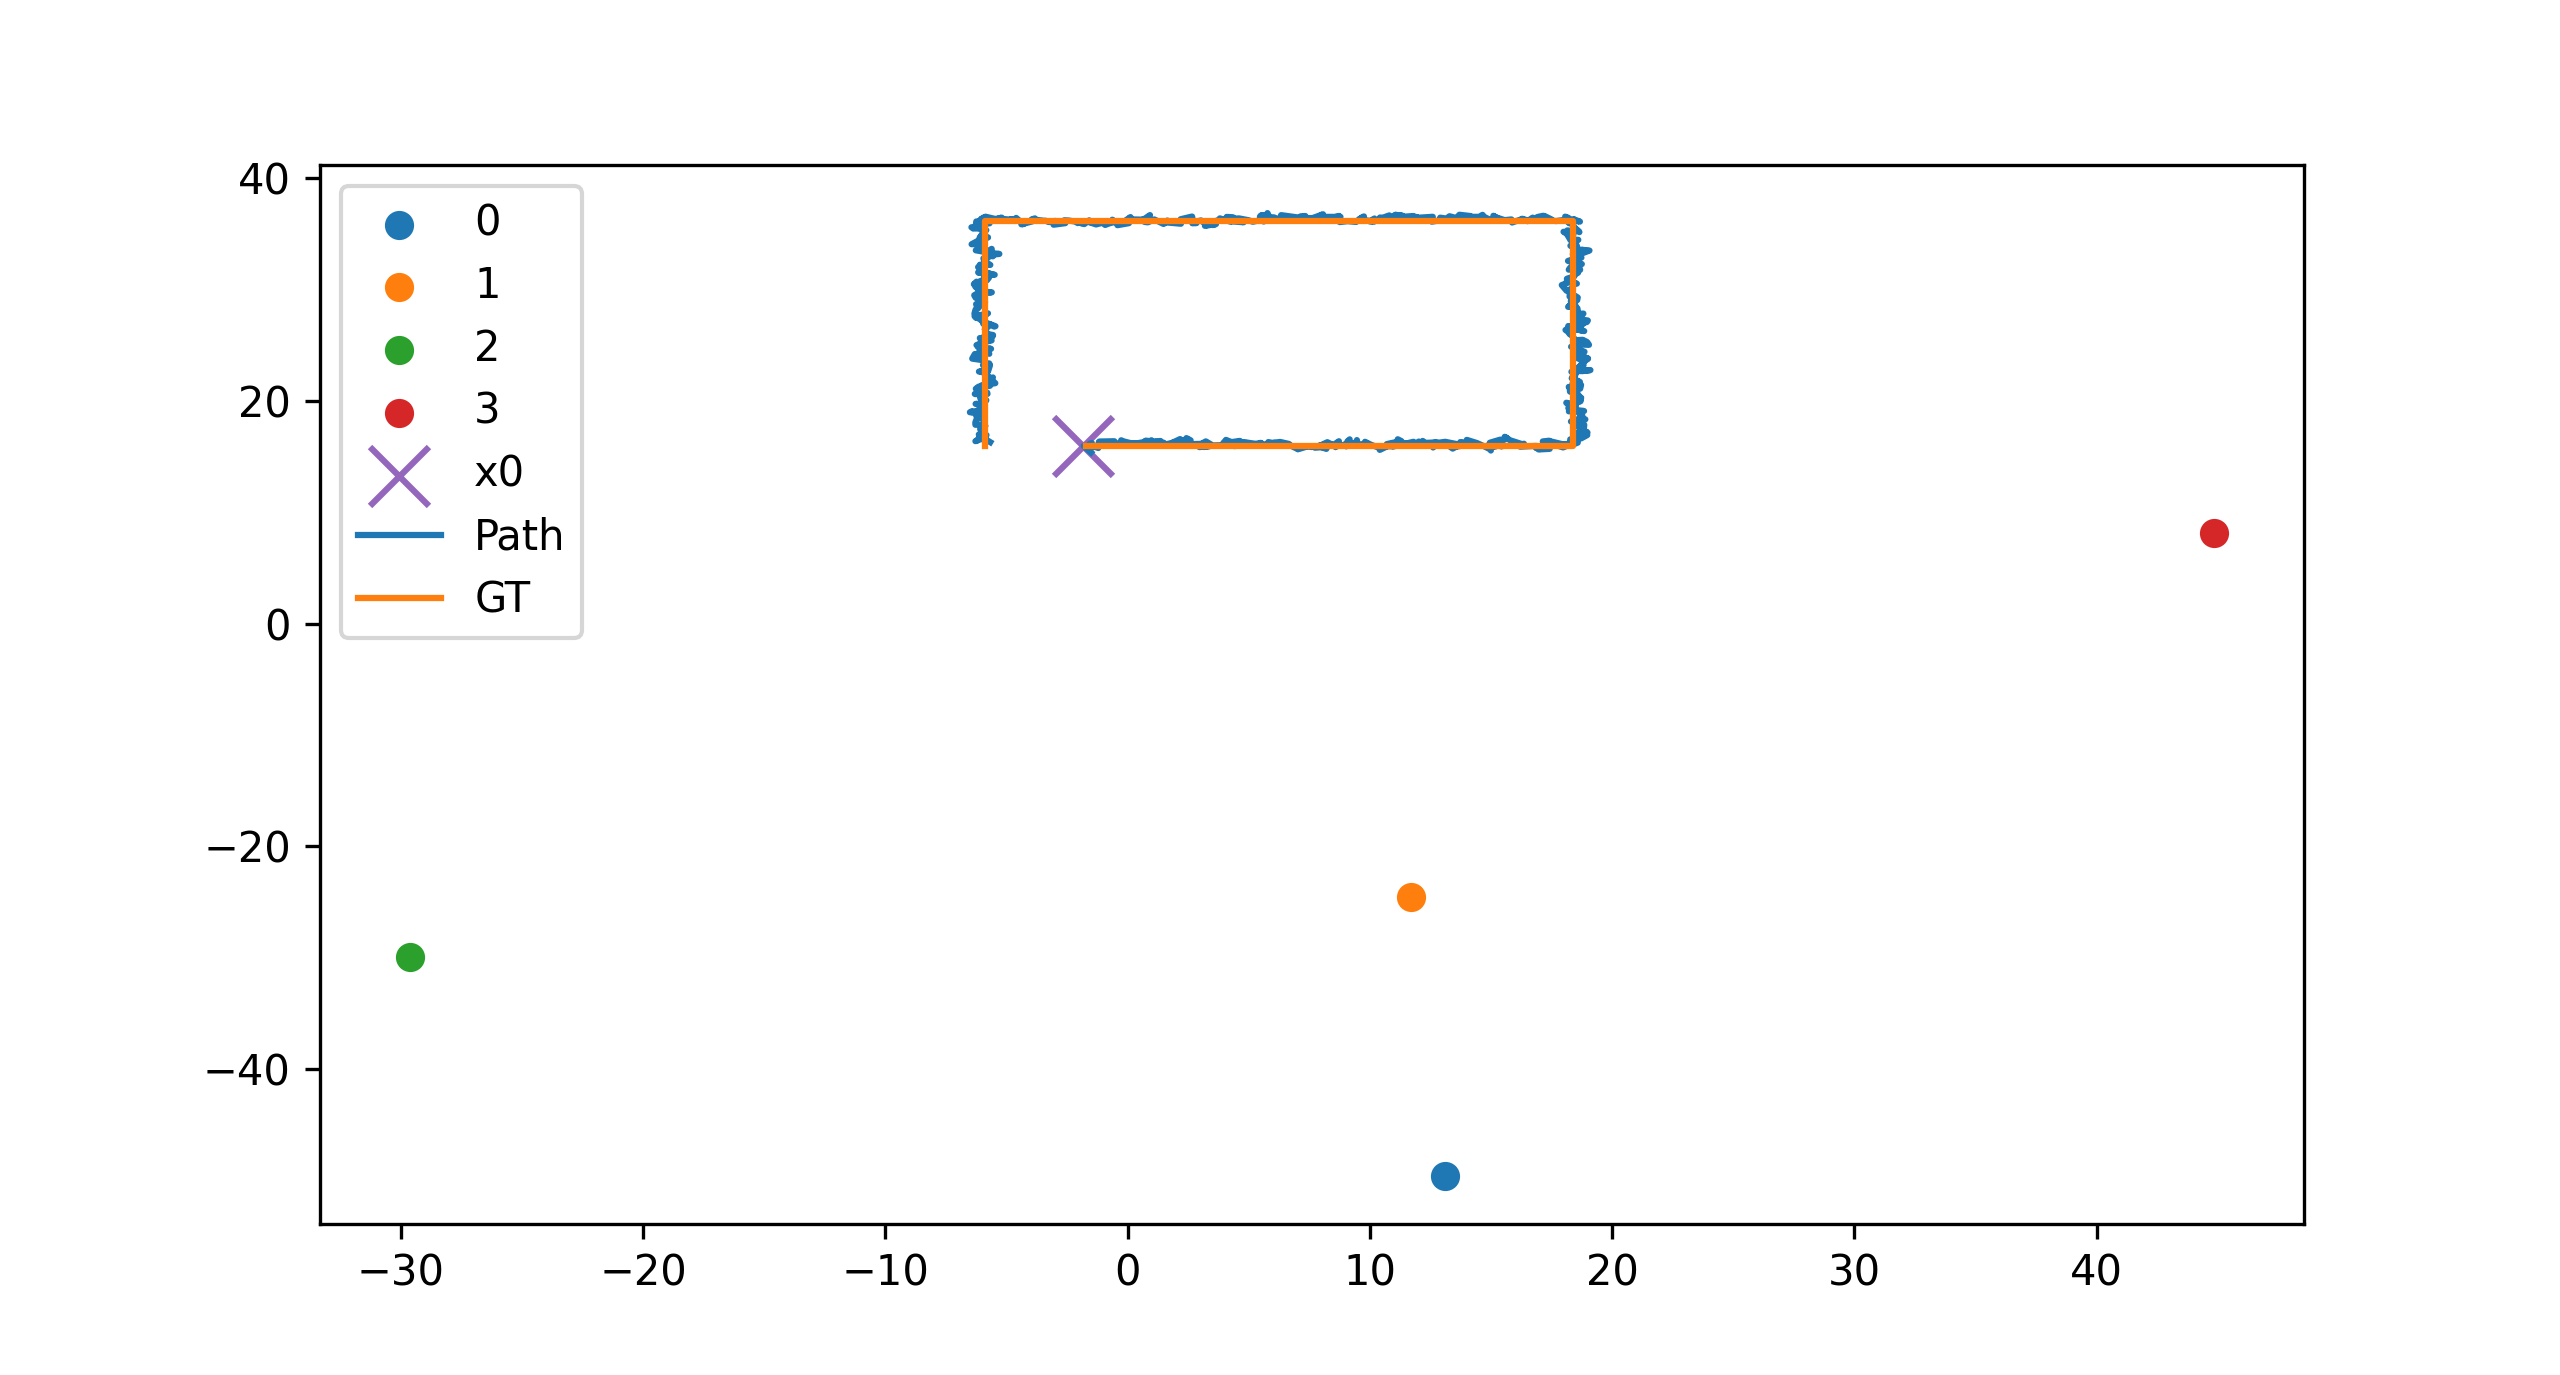
\includegraphics[width=\linewidth]{figures/sim.png}
    \caption{Simulation}
    \label{fig:sim}
\end{figure}

\subsection{Real-world experiments}

First, it's important to address the assumption made in the simulation environment. It was assumed that sensor measurement variance is known. For filter to have good convergence properties we would like to know it up to a reasonable accuracy level when in operation. Therefore, the first experiment was conducted to measure the precision of UWB range measurements compared to a ground truth. DTU ASTA's Opticon system was used to generate ground truth labels (limited to ~10m range) and two UWB devices, one configured as a tag and another one as an anchor. During the experiment anchor was moved to different position around the track, ground truth distance calculated between devices by taking norm of two position from Opticon and corresponding measurement by the means of UWB antennas was recorded. Figure \ref{fig:distancePDF} shows the probability distributions of measured values by real-world experiments in blue and the ground truth in orange.
\begin{figure}
    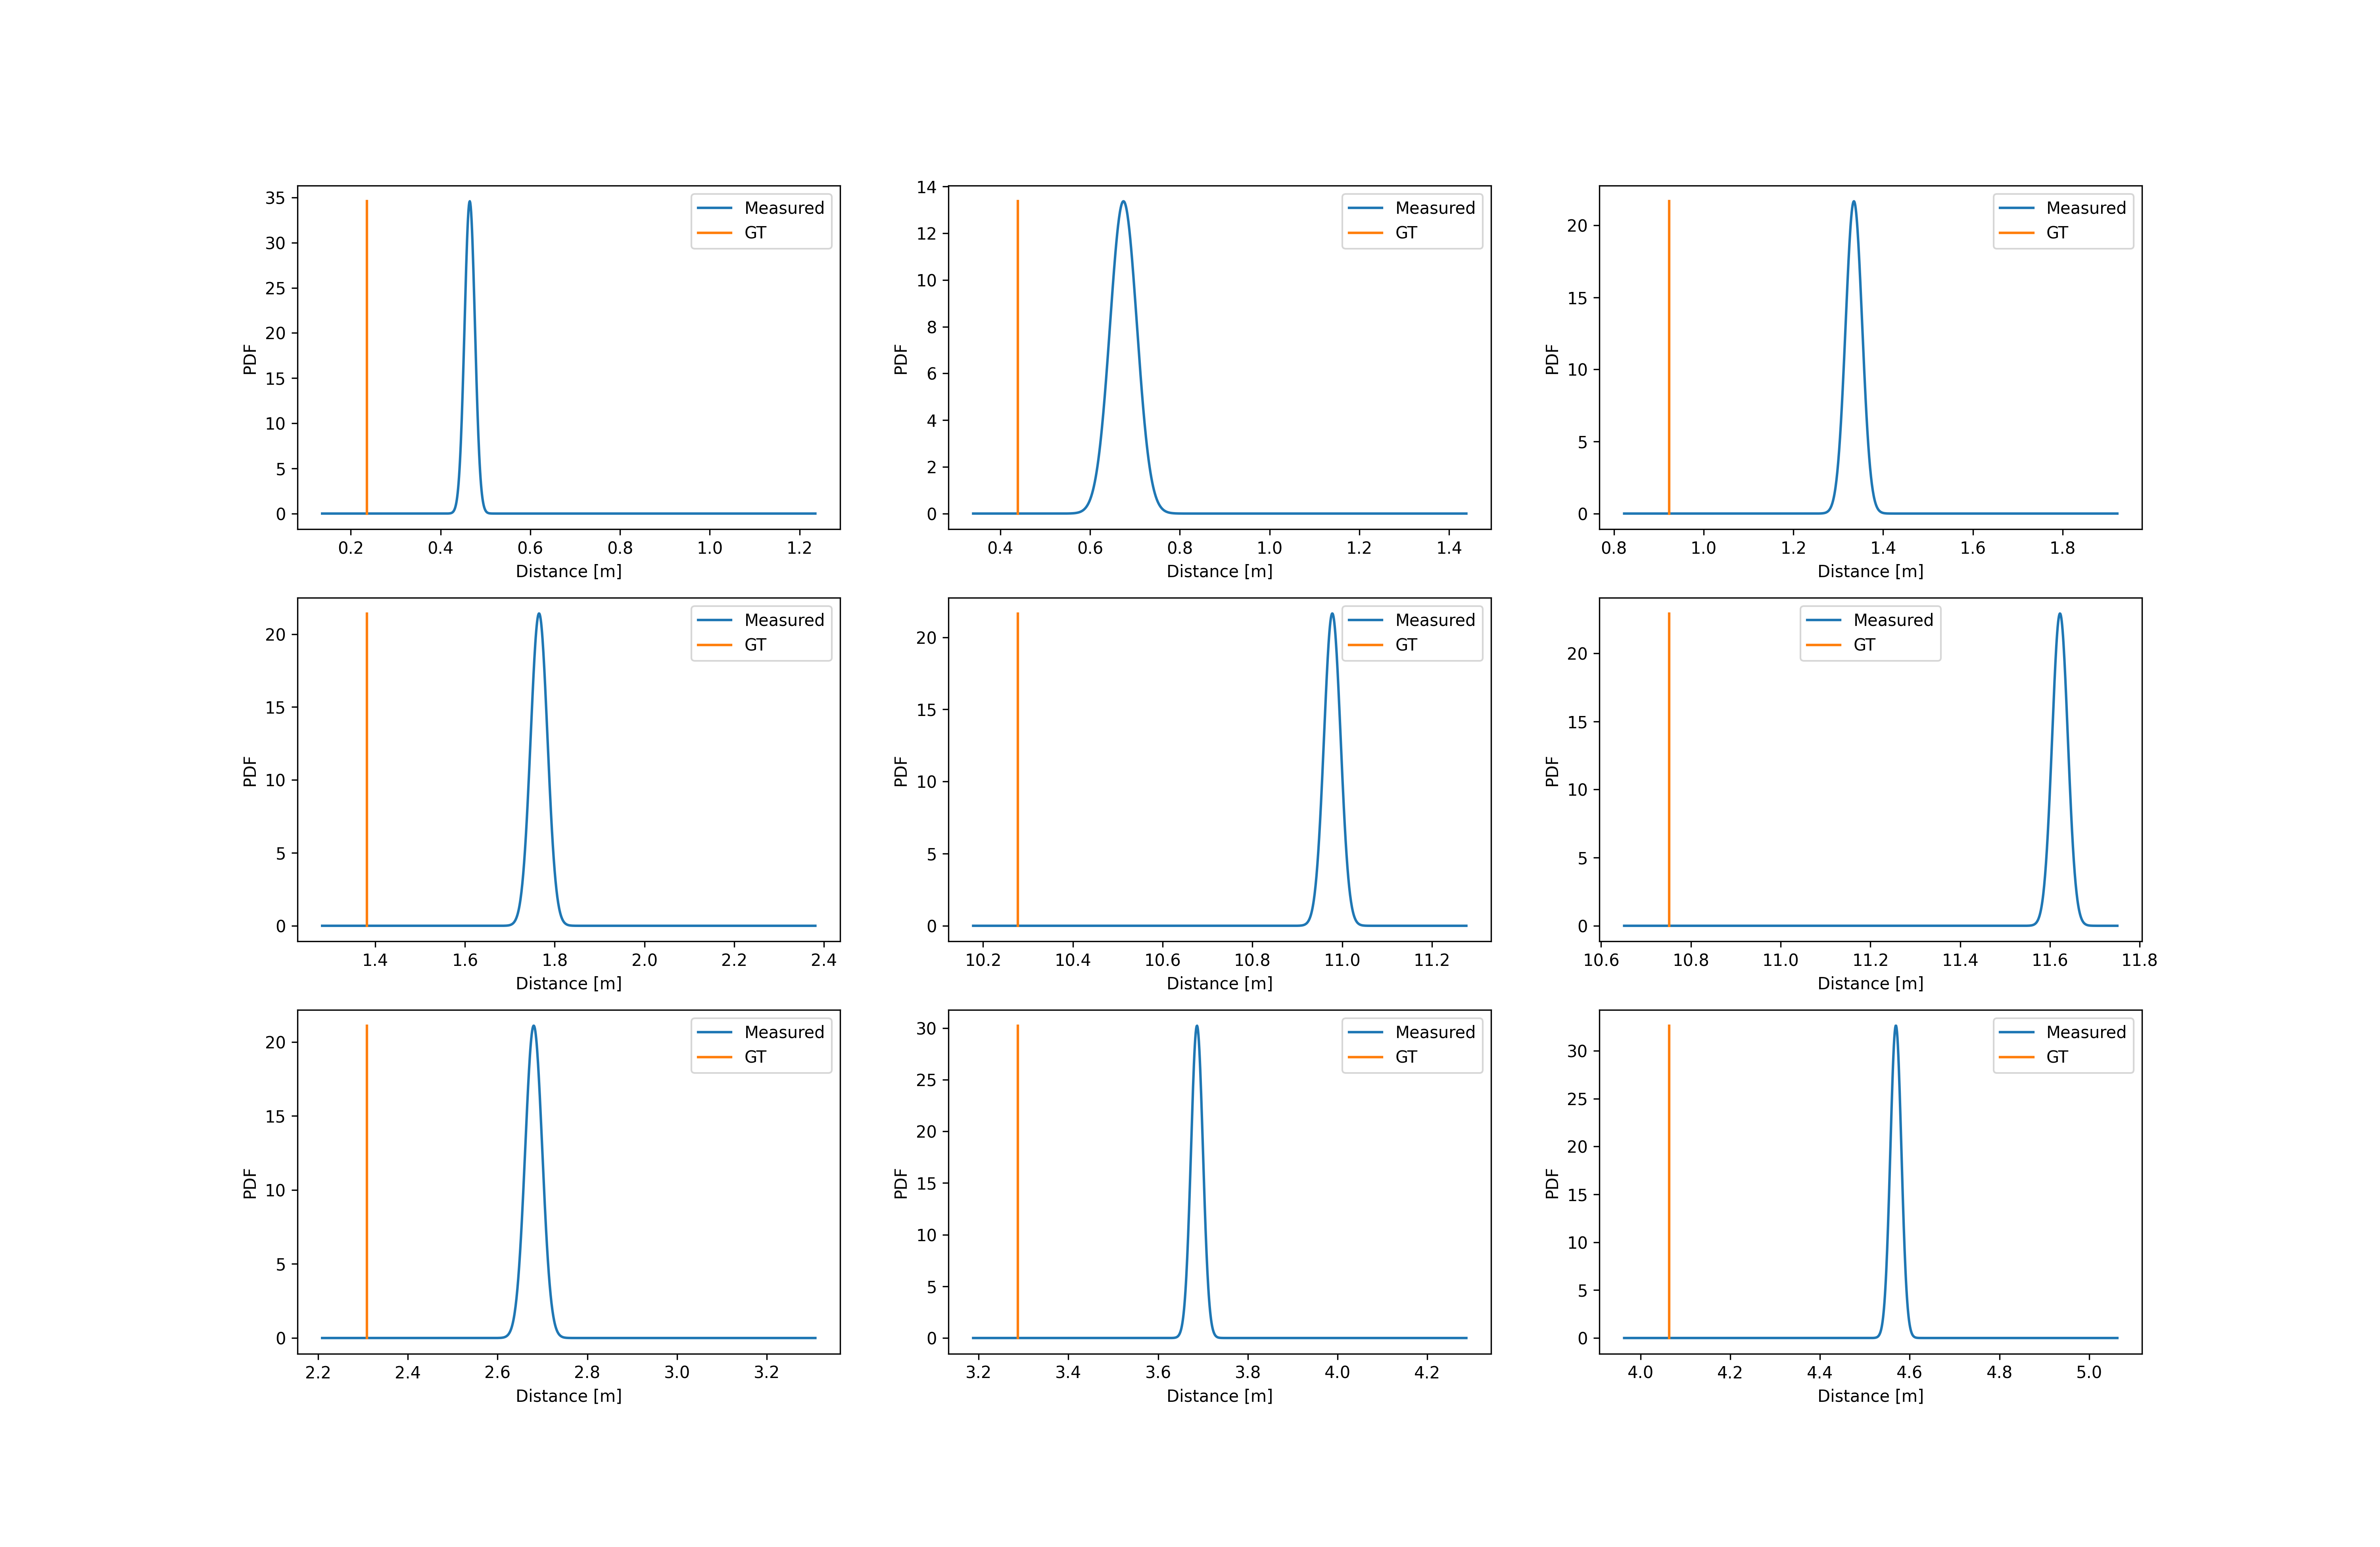
\includegraphics[width=\linewidth]{figures/distancePDF.png}
    \caption{Distance measurements PDFs.}
    \label{fig:distancePDF}
\end{figure}

Looking at the plots one noticeable thing is that mean value of measured values are shifted to the right - meaning sensor gives out bigger distance than it actually is, this could be called bias. The relationship of bias and distance is illustrated in Figure \ref{fig:distance_bias}. Additionally, it can be modeled, at least in this rang,  by a line fit, which is shown in the graph too. It approximates the bias reasonably well and will improve localization accuracy in this distance range. In a way, it's calibrating the sensor so that measurements have the same mean value as ground truths.
\begin{figure}
    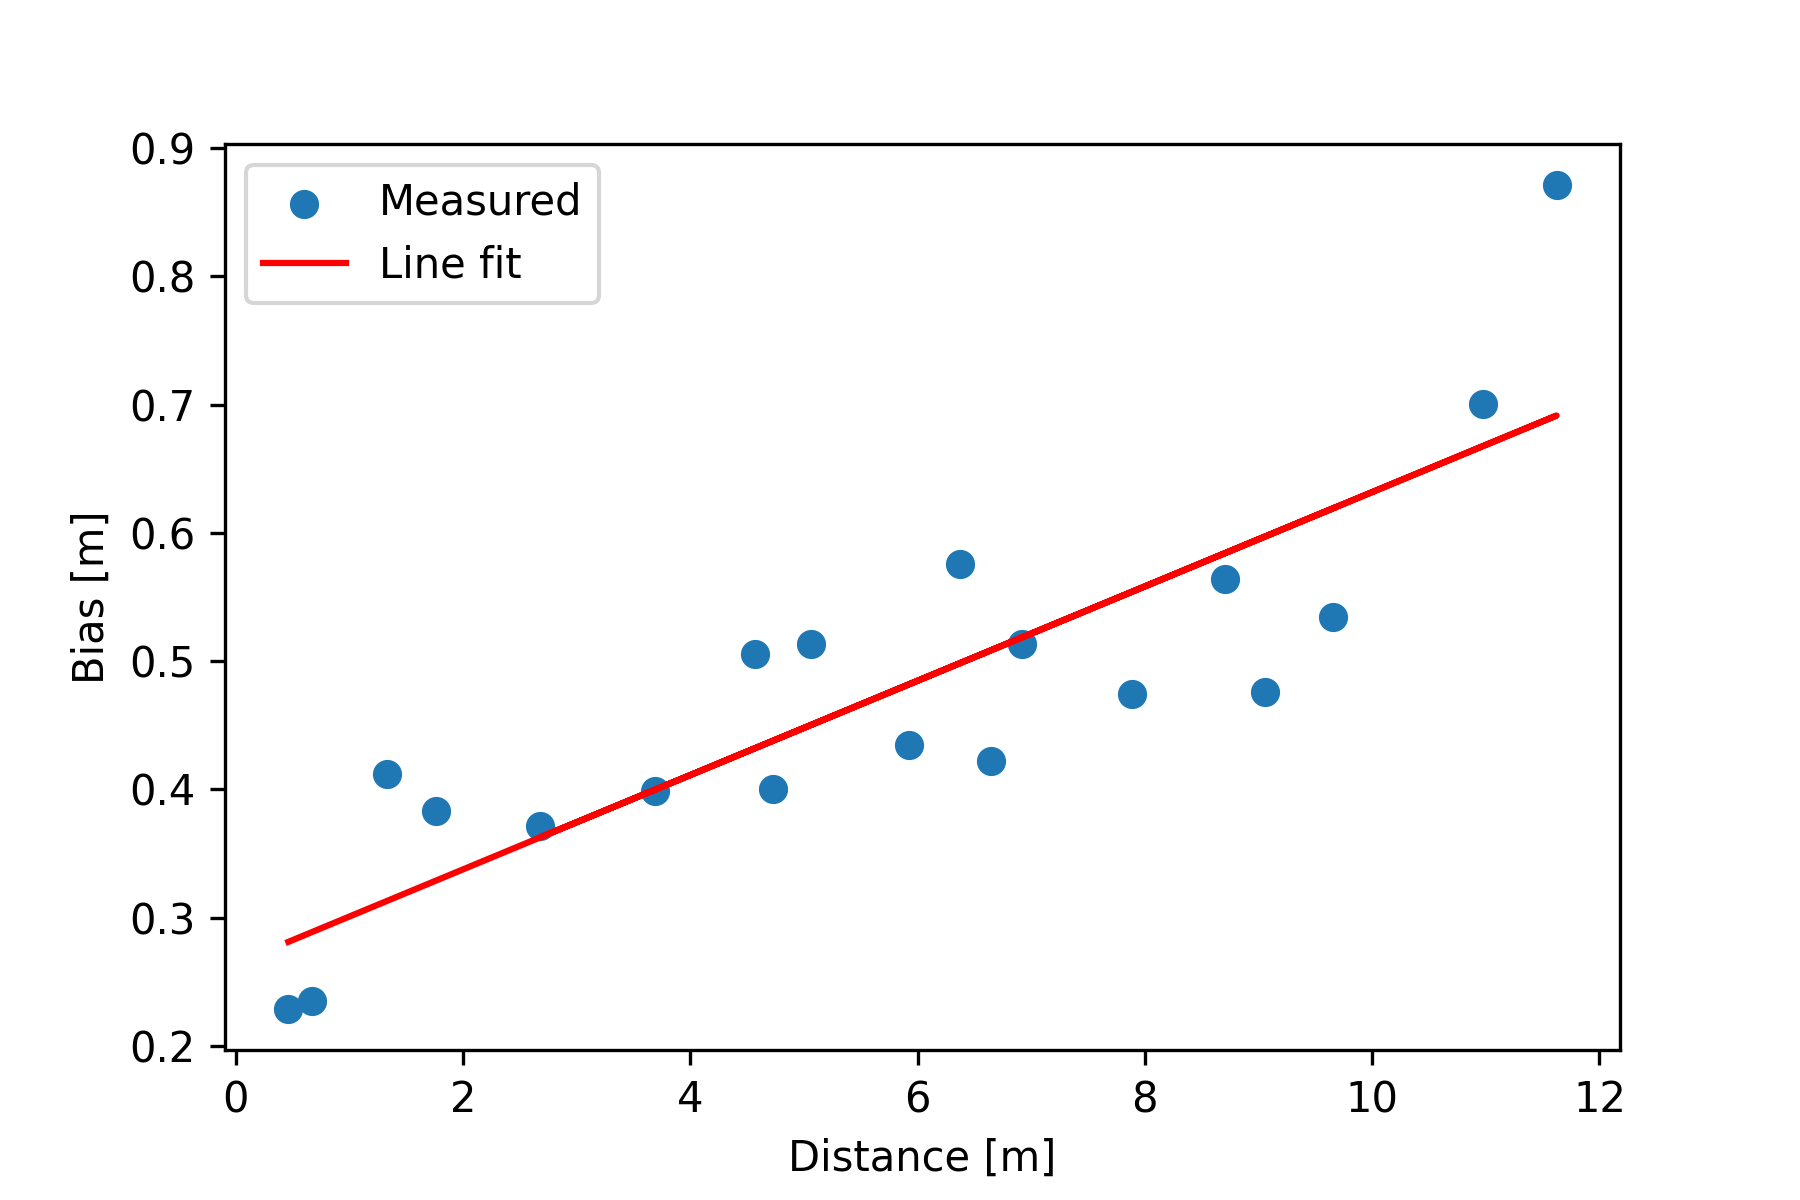
\includegraphics[width=\linewidth]{figures/distance_bias.png}
    \caption{Measurement bias over distance.}
    \label{fig:distance_bias}
\end{figure}

Next, let's look at the variance and distance relation. The question to ask here if they are dependant on each other or we can use single constant values for all range measurements. Figure \ref{fig:distance_var} shows them on single plot, plus a line fir on the data. It's clearly seen that variance is very low and of the same magnitude through out the data points. Thus, we can conclude that under tested conditions constant variance value can be used in EKF. For instance, an average value of all these variance points.
\begin{figure}
    \centering
    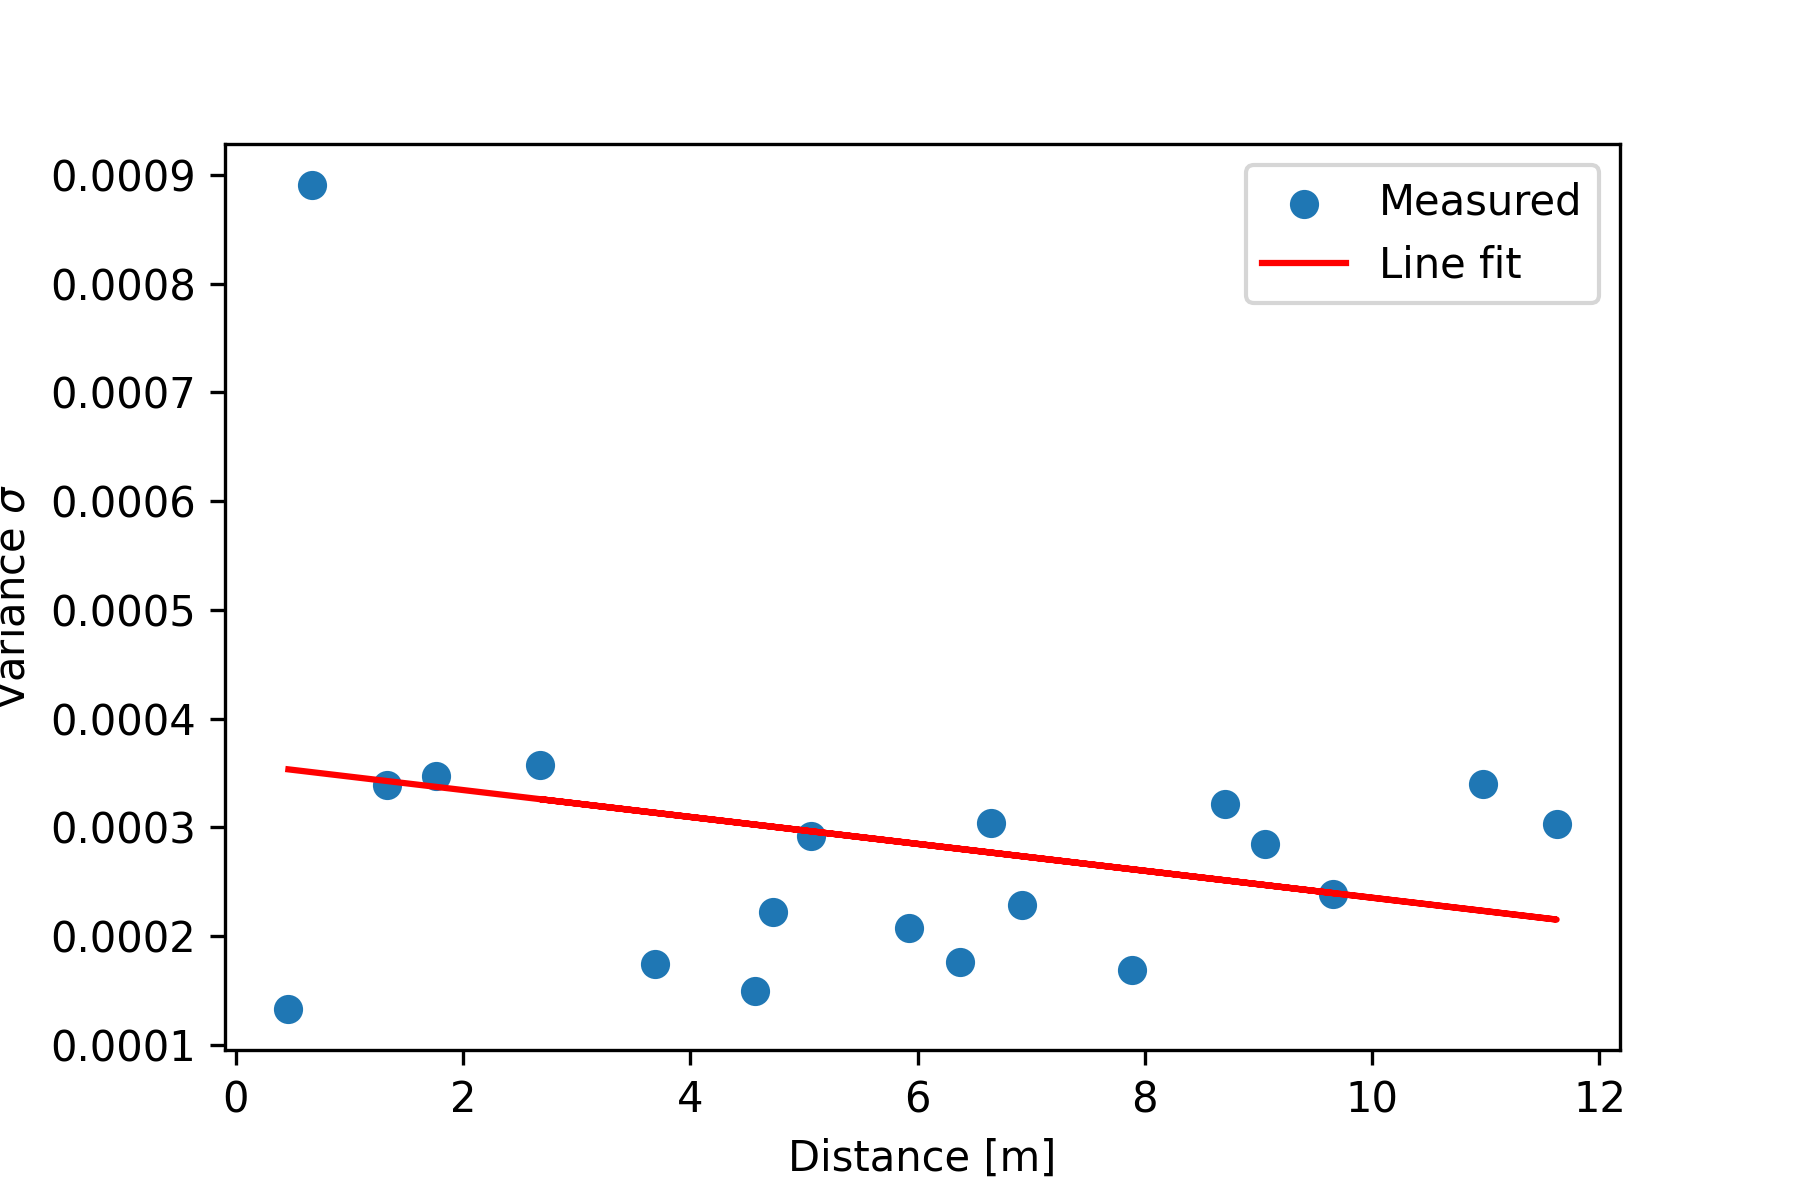
\includegraphics[width=\linewidth]{figures/dist_variance.png}
    \caption{Distance over measurement variance.}
    \label{fig:distance_var}
\end{figure}